\chapter{Introduction}

Production of integrated circuits has advanced at a consistent and rapid pace for over half a century, doubling the transistors density every one to two years in accordance with Moore's law. Only in recent years has the cadence has slowed as we approach fundamental physical limits.

While Moore's law is most commonly associated with improvements in performance, it has also allowed us to reduce the size of computers: doing the same thing in ever smaller packages. This trend has not been as smooth as the continuous improvements in performance. While any improvement in performance is a direct advantage, a small reduction in size usually isn't. However, at certain thresholds, it enables revolutions: moving from room-sized computers to home computers and PCs in every home,  scaling them down further to portable/laptop computers, and eventually handhelds and smart phones. Once established, each of these areas then benefitted from Moore's law to improve their capabilities, but the truly disruptive moments are when miniaturisation allowed whole new applications areas to emerge.

The term 'ubiquitous computing' was coined by Mark Weiser, predicting in 1991 that computing would move from a dedicated device on the desktop, to devices all around us, from alarm clocks to coffee makers \cite{Weiser:1991wz}. Around the turn of the century, we were able able to scale down useful, working devices to the size of a few millimetres \cite{Warneke:2001ui}. This led to the start of research into Wireless Sensor Networks (WSN): many small and inexpensive sensor nodes, often called 'motes', working together to perform continuous automated sensing tasks.

Many promising WSN applications were proposed, ranging from military applications \cite{Arora:2004}, to precision agriculture \cite{Langendoen:2006un}, habitat monitoring \cite{Mainwaring:2002wb}, and environmental monitoring \cite{WernerAllen:2006ta, Chang:2010ek}. While the applications vary greatly, the hardware platforms used to build WSN applications are all quite similar, and usually very resource-constrained.

Sensor nodes are small and battery powered, and many applications require a lifetime measured in weeks or months rather than hours, so maintaining a very low power consumption is critical. To achieve this, the CPUs used for sensor nodes are kept very simple. While they lack most of the features found in modern desktop CPUs, they typically do have several sleep modes, allowing them to reduce power consumption by over 99\%. Extremely long battery life is possible by keeping the CPU in sleep state for most of the time, only occasionally waking up to perform its sensing task. Since RAM requires power to maintain its state even in sleep mode, it is also limited, typically to only a few KB of RAM, a full six orders of magnitude less than most modern computers.

In 2001 Pister predicted that by 2010, the size of these devices would be reduced to a cubic centimetre, and cost to less than a dollar \cite{Pister:2001vr}. While the first prediction has come true \cite{Wang:2014cq}, the latter so far has not. Future improvements in IC technology may allow more powerful devices at the same level of cost and power consumption, but for many applications an increase in battery lifetime or a reduction in cost may be more valuable, and may enable new applications not possible at the current level of technology.

Thus, much of the research into WSN is about achieving useful functionality in as small a space as possible and the tradeoffs involved, gradually exploring the design space between capabilities, accuracy and performance on one side, and their cost in terms of memory and power consumption on the other.
%
To make these applications work new protocols were needed at every layer in an application, optimising them for the specific constraints of sensor nodes. This includes lightweight MAC protocols for radio communication trading latency for energy by turning off the radio as much as possible \cite{Ye:2002uv, vanDam:2018tr}, lightweight operating systems and virtual machines trading functionality for size and complexity \cite{Levis:2004ws, Gu:2006ww, Han:2005tha, Levis:2002ku, Brouwers:2009cj}, lightweight routing and data aggregation \cite{Intanogonwiwat:2018wz, Braginsky:2002wg}, lightweight data compression and reprogramming techniques trading CPU cycles for transmitted bits \cite{Marcelloni:2009ja, Reijers:2003ww}, lightweight localisation trading accuracy for complexity \cite{Niculescu:2001bl, Savarese:2002tx, Savvides:2002uf}, etc.

What these all have in common is that they revisit classing computer science problems, and adjust them to fit one a sensor node, making trade-offs to optimise for power consumption, either directly by reducing the time the processor or radio is active, or indirectly by reducing code size and memory consumption enough for them to run on the extremely low power, but also very resource-constrained CPUs.

\section{Internet-of-Things}
\label{sec-introduction-iot}
Recently, research into the Internet-of-Things (IoT) focusses on connecting many everyday objects and building smart applications with them. In this vision, similar to Weiser's ubiquitous computing, any object could be connected to the internet, and cooperate to achieve useful goals. For example a house with a smart airconditioning system may use sensors in each room, weather forecast information downloaded from the internet, past data on how the house responds to weather changes, and the user's current location, and combine all of this information to conserve energy and still make sure the house is at a comfortable temperature when the user gets home.

While IoT and WSN overlap and are sometimes used interchangeably, an important difference is that in WSN research applications typically consist of a large number of homogeneous and resource-constrained nodes, while IoT devices come in a wide range, with vastly different performance characteristics, cost, and power requirements.

On one end of the spectrum are devices like the Intel Edison and Raspberry Pi. These are the results of another decade of miniaturisation since the beginning of WSN research, and are basically a complete PC in a very small form factor. They are powerful enough to run a normal operating system like Linux, but relatively expensive and power hungry. On the other end are more traditional WSN CPUs like the Atmel Atmega or TI MSP430: much less powerful, but also much cheaper and low power enough to potentially last for months or years on a single battery. Since both classes of devices have such different characteristics, solutions that are appropriate for one, usually don't work for the other.

Another important difference between WSN and IoT applications is that in WSN applications the network is usually dedicated to a specific task and the hardware is an integral part of the design of the application. In the broadest IoT vision, a user's smart devices cooperate to implement new applications, but these may come from many different vendors and may not be specifically designed for the application a user may run. Coming back to the example from Weiser's paper \cite{Weiser:1991wz}, it is unlikely a user would be willing to buy a matching pair of a coffee maker and an alarm clock, just so that they will work together to have his coffee ready in the morning. The challenge for IoT is to allow a smart coffee maker and a smart alarm clock to be programmed in such a way to enable this application.

Thus, many IoT applications are inherently heterogeneous, and as Gu points out, even when powerful devices are used like the Raspberry Pi, it is not unusual for low power devices to be included to form a hybrid network and take advantage of their extremely long battery lifetime \cite{Gu:2006ww}. One of the main challenges then becomes how to programme these networks of IoT devices.



\section{Virtual machines}
The use of virtual machines has been common in desktop computing for a long time, with Java and .Net being the most well-known examples. There are several advantages to using VMs, the most obvious one being platform independence. Java enables a vast number of different models of Android phones to run the same applications. In a heterogenous environment as IoT applications are expected to be, a VM can significantly ease the deployment of these applications if the same programme can be sent to any node, regardless of it's hardware platform.

A second advantage is that a VM can offer a safe execution environment, preventing buggy or malicious code from disabling the device.

% A final often mentioned advantage is ease of programming. Many VMs allow the developer to write programmes at a higher level of abstraction than the bare-metal C programming that is still common for sensor nodes. However, it could be argued that this could also be achieved using more high level languages that compile to native code, so the two advantages of VMs that we will focus on in this thesis are safety and platform independent reprogramming.

Since the early days of WSN research, many sensor node VMs, some based on Java and .Net, have also been developed. They manage to pack an impressive set of features on such a limited platform, but almost all sacrifice performance.

\subsection{Performance}
\label{sec-introduction-performance}
The VMs for which we have found concrete performance data are shown in Table \ref{tbl-slowdown-for-sensornode-vms}. The best case, the 'only' 4x slowdown in one of SensorScheme's benchmarks, is a tiny benchmark that just calls a random number generator, so this only tells us a function call costs about 3 times longer than generating the random number. Apart from this single data point, all interpreting VM are between one and two orders of magnitude slower than native code.

\begin{table*}[]
\centering
\caption{Slowdown for interpreting sensor node VMs.}
\label{tbl-slowdown-for-sensornode-vms}
\begin{tabular}{lllr}
\toprule
VM              & Source                           & Platform                   & Performance vs native C \\
\midrule
Darjeeling      & Delft University                 & ATmega128                  & 30x-113x slower \cite{Brouwers:2009cj} \\
                & ~~ of Technology                 &                            & \\
TakaTuka        & University of Freiburg           & Mica2 (AVR) and            & 230x slower \cite{Ellul:2012thesis} \\
                &                                  & JCreate (MSP)                           & \\
TinyVM          & Yonsei University                & ATmega128                  & 14x-72x slower \cite{Hong:2009gc} \\
DVM             & UCLA                             & ATmega128L                 & 108x slower \cite{Balani:2006} \\
                &                                  &                            & 500x slower \cite{Kumar:2007ge} \\
SensorScheme    & University of Twente             & MSP430                     & 4x-105x slower \cite{Evers:2010ur} \\
                &                                  &                            & \\
% Ellul's work \cite{Ellul:2012thesis}    & University of Southampton       & MSP430                     & 2.2x-9x slower           \\
\bottomrule
\end{tabular}
\end{table*}

In many scenarios this may not be acceptable for two reasons: for many tasks such as periodic sensing there is a hard limit on the amount of time that can be spent on each measurement, and an application may not be able to tolerate a slowdown of this magnitude. For applications that sample close to the maximum rate a node could process, any reduction in performance directly translates to a reduction in the sampling rate.

Perhaps more importantly, one of the main reasons for using such tiny devices is their extremely low power consumption. In many applications the CPU is expected to be in sleep mode most of the time, so little energy is be spent in the CPU compared to communication, or sensors.

But if the slowdown incurred by a VM means the CPU has to stay in active mode 10 to 100 times longer, this means 10 to 100 times more energy is spent on the CPU and it may suddenly become the dominant factor and reduce battery lifetime. To illustrate this we will look at two concrete examples below.

\paragraph{Mercury}
Few applications report a detailed breakdown of their power consumption, but one that does is Mercury \cite{Lorincz:2009kt}, a platform for motion analysis. The data reported in their paper is copied in Table \ref{tbl-mercury-energy}. The greatest energy consumer is the sampling of a gyroscope, at 53163 uJ. Only 1664 uJ is spent in the CPU on application code for an activity recognition filter and feature extraction. When multiplied by 10 or 100 however, the CPU becomes a very significant, or even by far the largest energy consumer.

\begin{table*}[]
\centering
\caption{Energy consumption breakdown for the Mercury motion analysis application. (source: \cite{Lorincz:2009kt})}
\label{tbl-mercury-energy}
\begin{tabular}{lr}
\toprule
Component                          & Energy (uJ) \\
\midrule
\small
Sampling accel                     &  2805 \\
CPU (activity filter)              &   946 \\
Radio listen (LPL, 4\% duty cycle) &  2680 \\
Time sync protocol (FTSP)          &   125 \\
Sampling gyro                      & 53163 \\
Log raw samples to flash           &  2590 \\
Read raw samples from flash        &  3413 \\
Transmit raw samples               & 19958 \\
\midrule
Compute features                   &   718 \\
Log features to flash              &    34 \\
Read features to flash             &    44 \\
Transmit features                  &   249 \\
\midrule
512-point FFT                      & 12920 \\
\bottomrule
\end{tabular}
\end{table*}


Table \ref{tbl-mercury-energy} also shows us that transmitting raw data is a major energy consumer. To reduce this, Mercury has the option of first extracting features from the sensor data, and transmitting these instead, achieving a 1:60 compression. Mercury has five feature detection algorithms built in: maximum peak-to-peak amplitude; mean; RMS; peak velocity; and RMS of the jerk time series. But they note that the exact feature extractor may be customised by an application.

This is the kind of code we may want to update at a later time, where using a VM could be useful to provide safety and platform independence. However, at a 10x to 100x slowdown in the feature extraction algorithm this would not work anymore, since more energy would then be spent in the CPU than we would save on transmission.

Finally, a more complex operation such as a 512 point FFT costs 12.920 mJ. For tasks like this, even a slowdown by a much smaller factor will have a significant impact on the total energy consumption.

\paragraph{Lossless compression}
As a second example we consider lossless data compression. Since the radio is typically one of the major power consumers on mobile devices, compressing data before it is sent is an attractive option to conserve energy spent on transmission, but energy must also be spent on the CPU during (de)compression. Barr and Asanovi\ ́c have analysed this tradeoff for five compression algorithms on the Skiff research platform, with hardware similar to the Compaq iPAQ. They found the break-even point to be at about 1000 instructions for each bit saved. Beyond that the energy spent on compression would start to outweigh the energy saved on transmission. They found a number of cases where this was the case, and using some compression algorithms would increase total energy consumption, compared to sending uncompressed data \cite{Barr:2006vg}.

Most of the traditional algorithms considered by they Barr and Asanovi\ ́c are too complex to run on a sensor node, so specialised compression algorithms have been developed for sensor nodes. One such algorithm is LEC \cite{Marcelloni:2009ja}, a simple lossless compression algorithm that can be implemented in only a few lines of code and only needs to maintain a few bytes of state. We will use a rough calculation to show why performance is also a concern for the simpler compression algorithms developed for sensor nodes.

%TODO: check these calculations
Using the power consumption from the datasheets for the Atmel ATMEGA128 \cite{Atmel:ATMEGA128Datasheet} CPU, we determine the energy per cycle. Running at 8 Mhz and 2.7V, the ATMEGA consumes 7.5mA.

\begin{equation}
	7.5mA * 2.7V / 8MHz = 2.53nJ / cycle  
\end{equation}

We can do a similar calculation to determine the energy per bit for the Chipcon CC2420 radio.  This radio can also operate at 3V, and consumes between 8.5 and 17.4 mA depending on transmission power. Using the higher value, so that compression will be more worthwhile, this yields

\begin{equation}
  17.4mA * 2.7V / 250kbps = 187.9nJ / bit
\end{equation}

As a result, we can spend $187.9/2.53 \approx 74$ cycles per bit to reduce the size of the transmitted data, and still conserve energy.

We implemented the LEC compression algorithm and used it to compress a dataset of 256 16-bit ECG measurements \cite{physionet-ecg-data}, or 4096 bits of data. The results are shown in Table \ref{tbl-lec-energy}. LEC compression reduced the dataset to 1840 bits, saving 2256 bits, or 424 uJ on transmitting the data, at the expense of 246 uJ extra energy spent in the CPU.

\begin{table}[H]
\centering
\caption{LEC compression energy savings}
\label{tbl-lec-energy}
\begin{tabular}{lr}
\toprule
%// component                          & energy (uJ) \\
\midrule
ATMEGA128 energy per cycle            & 2.53 nJ/cycle  \\
CC2420 energy per transmitted bit     & 187.9 nJ/cycle  \\
\midrule
LEC compression cycles spent          & 97052 cycles\\
LEC compression bits saved            & 2256 bits \\
LEC compression cycles per bit        & 43 cycles/bit \\
~~~ energy expended                   & 246 uJ \\
~~~ energy saved                      & 424 uJ \\
~~~ ratio saved/expended              & 1.7x \\
\bottomrule
\end{tabular}
\end{table}

This shows that for this combination of hardware and sensor data, LEC compression is effective in reducing total energy consumption. However the energy saved is only 1.7x more than the extra energy expended on the CPU. This means that if the slowdown from running this in a VM is more than 1.9, and thus time and energy spent on the CPU increases by a factor larger than 1.9, this would tip the balance in favour of just sending the raw data.

Where exactly the break-even point lies depends on many factors. The CPUs and radio used in this calculation are very common in typical sensor nodes, for example the widely used Telos platform \cite{Polastre:2005ut} is based on the CC2420 radio and the ATMEGA cpu is found in many Arduinos. However many parameters will affect the results. Power consumption is roughly linear in relation to clock frequency, so at the same voltage the cost per cycle will be similar, but at lower frequencies the CPU can operate at a lower voltage which lowers the cost per cycle. The cost per bit depends on many factors including the link quality. A bad link will increase the cost per bit due to retransmissions, but if the node chooses to transmit at a lower power, for example to reduce the number of neighbours and collisions, the cost per bit will be lower than calculated.

This calculation is only meant to indicate that there are many situations where the slowdown caused by current sensor node VMs will be an issue. For Mercury's feature extraction, the break-even point is around 27x slowdown, while for this case of LEC compression it is at only 1.9x. While the exact numbers depend on the application, it is clear that a slowdown of one to two orders of magnitude will affect battery lifetime in many cases.

\paragraph{Ahead of time compilation}

Thus, a better performing VM is needed, preferably one that performs as close to native performance as possible. Translating bytecode to native code is a common technique to improve performance in desktop VMs. Translation can occur at three moments: offline, ahead-of-time (AOT), or just-in-time (JIT). JIT compilers translate only the necessary parts of bytecode at run-time, just before they are executed. They are common on desktops and on more powerful mobile environments, but are impractical on sensor node platforms that can often only execute code from flash memory. This means a JIT compiler would have to write to flash memory at run-time, which is expensive and would cause unacceptable delays. Translating to native code offline, before it is sent to the node, has the advantage that more resources are available for the compilation process. We do not have a JVM compiler that compiles to our sensor node's native code to test the resulting performance, but we would expect it would be similar to compiled C code. However, doing so, even if only for small, performance critical sections of code, sacrifices the two of the key advantages of using a VM: The host now needs knowledge of the target platform, and needs to prepare a different binary for each type of CPU used in the network, and for the node it will be difficult to provide a safe execution environment when it receives binary code.

Therefore, this thesis will focus on the middle option: translating the bytecode to native code on the device itself, at load time. We will build on previous work by Joshua Ellul \cite{Ellul:2012thesis} on AOT translation on sensor nodes, which resulted in a reduction in performance overhead to a slowdown of up to 9x, but also resulted in an increase in the size of the stored programmes of up to 4.5x, limiting the size of the programmes that can be loaded on a device.

\subsection{Safety}
\label{sec-introduction-safety}
Low-cost low-power sensor node CPUs have a very simple architecture. They typically do not have a memory management unit (MMU) or privileged execution modes to isolate processes. Instead, the entire address range is accessible from any part of the code running on the device.

At the same time, sensor node code can be complex. While programming in a high-level language can reduce the risk of programming errors, the limited resources on a sensor device still often force us to use more low-level style approaches to fit as much functionality and data on a device, for example by storing data in simple byte arrays instead of using more expensive objects. In such an environment, mistakes are easily made, and with full access to the entire address space can have catastrophic consequences. A second threat comes from malicious code. As IoT applications become more widespread, so do the attacks against them, and the unprotected execution environment of sensor node CPUs makes them an attractive target.

To guard against both buggy code and malicious attacks, a desirable property would be the ability to execute code in a sand boxed manner and isolate untrusted application code from the VM itself. Specifically, we would like to guarantee that malicious code cannot:
\begin{enumerate}
	\item write to memory outside the range assigned by the VM
	\item perform actions it does not have permission for
	\item retain control of the CPU indefinitely
\end{enumerate}

Note that these guarantees do not say anything about the correctness of the application itself: buggy code may still corrupt it's own state. More fine-grained checks can be useful to reduce the risk of bugs and speed up the development process by detecting them earlier. Safe TinyOS \cite{Cooprider:2007ub} adds runtime checks to detect illegal writes, and can do so efficiently by analysing the source code before it is compiled. However, this doesn't protect against malicious code being sent to the device and depends on the correctness of the host.

Our approach depends only on the correctness of our VM, and guarantees it can always regain control of the node and terminate any misbehaving application before it executes an illegal write or performs an action it is not permitted to.


\section{Scope}
\label{sec-introduction-scope}
Internet-of-Things devices come in a wide range with varying capabilities. The larger IoT platforms are powerful enough to run standard operating systems, tools and languages, and VMs are well established as a good way to programme devices powerful enough to run advanced JIT compilers. This thesis focusses specifically on small sensor nodes for which no such standards exists. These platforms have the following characteristics:
\begin{itemize}
	\item Split data and programme memory: RAM for data, and flash memory for code are separated. While some device can execute code from both RAM and flash \cite{TexasInstrumentsIncorporated:MSP430F1611Datasheet}, others cannot \cite{Atmel:ATMEGA128Datasheet}.
	\item Very limited memory: Since RAM consumes energy even when the CPU is in sleep mode, it is typically restricted to 10 KB of RAM or less. More flash memory is usually available to hold programmes, but at 32-256KB this is still very limited.
	\item Simple CPUs: While usually rich in IO to drive actuators and read from sensors, the rest of the CPUs used in these devices is usually a very simple RISC design to save cost and power consumption. Instructions usually take a fixed number of cycles, since memory is on chip access times are constant and fast, and there are no complicating factors like pipelines, caches, or branch predictions to consider.
	\item Very limited energy budget: Typical usage scenarios for WSNs demand a long battery lifetime, since frequent replacement or recharging would be too impractical or costly. All aspects of WSN software design are therefore focused towards minimizing energy use.
\end{itemize}

Our focus on sensor nodes raises the question of how platform independent our VM is, since IoT applications may mix both classes, and the ability to use a single binary to programme multiple classes of devices is exactly one of the advantages of using a VM. While the optimisations we propose are specifically developed to work in a resource constrained sensor device, the bytecode is very close to standard Java, so a more powerful device would have no problem running it just as efficiently as it runs normal Java code.

\begin{figure}[]
  \centering
  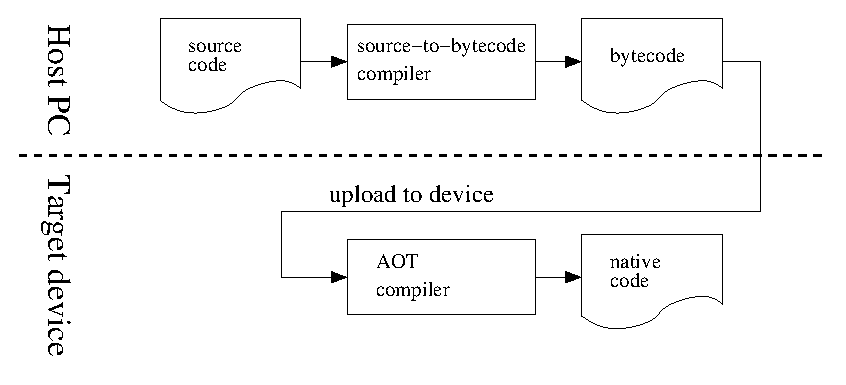
\includegraphics[width=0.6\linewidth]{compilation-process-highlevel.eps}
  \caption{Highlevel overview of the compilation process}
  \label{fig-compilation-process-highlevel}
\end{figure}

\paragraph{AOT compiler}
Figure \ref{fig-compilation-process-highlevel} shows the high level compilation process. The host PC will compile some source code to bytecode, which is uploaded to the target node. Instead of interpreting this bytecode, our VM will translate it at load time, and then execute the resulting native code.

We will see that in order to achieve good performance, an optimising compiler to generate high quality bytecode is necessary. However, the focus in this thesis is on developing techniques for the AOT compiler running on the sensor node. We want to examine what kind of performance it can deliver, given good quality bytecode.

Although we will make some changes to the way the bytecode is produced, building a full optimising compiler is clearly outside the scope of this thesis, but we will do some manual optimisations that we are confident an optimising compiler could do automatically to determine what level of performance is possible.

\paragraph{Source language}
Note that in Figure \ref{fig-compilation-process-highlevel} we use anonymous 'source code' and 'bytecode' instead of Java or JVM bytecode, since the use of Java was only motivated by the availability of existing work to build upon, most notably Darjeeling VM \cite{Brouwers:2009cj}, not because we believe Java to be a particularly good choice.

The question we wish to answer is not "How well can \emph{Java} run on a sensor node?", but "How well can a VM providing \emph{platform independence and safety} run on a sensor node?", and "What should a VM specifically designed for sensor nodes look like?"

We will see that in fact Java, in its current form, is nearly unusable for serious applications, and will end with a number of suggestions on how to remedy these issues.


\section{Research questions and contributions}
\label{sec-introduction-research-questions}
The main focus of this thesis is on assessing the suitability of VMs as a means to programme sensor node devices. The main research questions we will answer are:
\begin{itemize}
	\item How close can an AOT compiling sensor node VM come to native C performance?
	\item What are the tradeoffs?
	\item Can a VM be an efficient way to provide a safe, sandboxed execution environment on a sensor node?
	\item Is Java a suitable language for a sensor node VM, and how may it be improved?
\end{itemize}

Specifically, this thesis makes the following contributions:
\begin{itemize}
	\item We identify the major sources of overhead when using the baseline approach to AOT compilation, as described by Ellul and Martinez \cite{Ellul:2010iw, Ellul:2012thesis}.
	\item Using the results of this analysis, we propose a set of optimisations to address each source of overhead, including a lightweight alternative to Java method invocation to reduce method call overhead.
	\item These optimisations eliminate most of the performance overhead caused by the JVM's stack-based architecture, and over 80\% of performance overhead overall.
	\item They also reduce the code size overhead by 56\%, and show that the increase in VM size is quickly compensated for, thus mitigating a drawback of the previous AOT approach.
	\item We show that besides these improvements to the AOT technique, better optimisation in the Java to JVM bytecode compiler is critical to achieving good performance.
	\item We describe a number of checks that are sufficient for the VM to provide our desired safety guarantees, and show how most of these checks can be easily done at load time, reducing the overhead of run-time checks.
	\item We provide a comprehensive evaluation to analyse the overhead and the impact of each optimisation, and to show these results hold for a set of benchmarks with very different characteristics, including the commonly used CoreMark benchmark \cite{coremark}, and a number of benchmarks with typical sensor node code.
	\item Using the same benchmarks we evaluate the cost of our safety checks, and show this to be comparable or better than two existing approaches to provide a safe execution environment on a sensor node.
	\item Finally, we identify a number of aspects of the Java virtual machine that make it a bad match for sensor nodes, and propose ways to address these issues in future sensor node VMs.
\end{itemize}

\section{Structure of thesis}
Chapter 2 introduces some necessary background knowledge on wireless sensor networks, Java and the Java virtual machine, and JIT and AOT compilation.

Chapter 3 discusses the state of the art in improving performance for sensor node VMs and providing safe execution environments.

Chapter 4 describes the global design of MyVM.

Chapter 5 first analyses the sources of overhead for the current state of the art in sensor node AOT compilers, and then presents a set of optimisations to address each of these sources. In a number of cases where there were multiple options to implement an optimisation we also describe alternatives and motivate our choice.

Chapter 6 presents a set of checks that allow MyVM to provide the sandbox safety guarantees described in Section \ref{sec-introduction-safety}, and shows how the JVM's simple design allows for most of these checks to be done at load time.

Chapter 7 evaluates the effect of the optimisations presented in Section \ref{sec-optimisations} and the cost of the safety checks presented in Section \ref{sec-safety} and compares this with related work on safe execution environments. We use a set of benchmarks with different characteristics, both synthetic ones to show the behaviour in extreme cases and several benchmarks taken from real sensor node code.

Chapter 8 describes a number of issues we encountered while doing this work, which show Java in its current form is not the best choice for a sensor node VM, and suggests ways to improve these in future sensor node VMs.

Chapter 9 concludes this work.

\section{List of publications}
This dissertation is based on previously published technical reports or conference proceedings. The material presented in the subsequent chapters is based on the content of these publications.

\begin{itemize}
	\item N. Reijers, K. J. Lin, Y. C. Wang, C. S. Shih, and J. Y. Hsu, “Design of an Intelligent Middleware for Flexible Sensor Configuration in M2M Systems”, 2nd International Conference on Sensor Networks (SENSORNETS), Feb. 2013.
	\item N. Reijers and C.-S. Shih, “Ahead-of-Time Compilation of Stack-Based JVM Bytecode on Resource-Constrained Devices”, International Conference on Embedded Wireless Systems and Networks (EWSN), Feb. 2017.
	\item N. Reijers and C.-S. Shih, “Improved Ahead-of-Time Compilation of Stack-Based JVM Bytecode on Resource-Constrained Devices,” arXiv:1712.05590, Dec. 2017.
\end{itemize}

\section{Naming}
In literature various names are used for our target devices. The word \emph{mote} was common in early WSN research, as was \emph{sensor node}, or \emph{device} although the latter may also refer to larger, more powerful devices. In this thesis we will use the terms \emph{sensor node} or simply \emph{node} interchangeably to refer solely to the type of severely resource-constrained devices described above.

The terms \emph{wireless sensor networks}, \emph{cyber-physical systems} and \emph{internet-of-things} are all commonly used to describe sensor node applications. We will use WSN since it is the longer established term, and more clearly focussed on resource-constrained devices, but note that this also covers a large portion of IoT applications.

When reprogramming these devices, the code is expected to be sent by a more powerful device in charge of configuring the network. These more powerful devices outside or on the edge of wireless sensor network are refered to in literature by various names, including \emph{server}, \emph{gateway}, \emph{master}, \emph{controller}, or \emph{host}. While these names have slightly different accents or refer to different roles, this is not relevant for the work in this thesis. We will use \emph{host} to refer to the source of the code that is uploaded to the sensor node, possibly over multiple hops in the network, and assume the host to be a more powerful device with desktop-class processing capabilities.


